\documentclass[tikz,border=10pt]{standalone}
\usepackage[utf8]{inputenc}
\usepackage[T1]{fontenc}
\usepackage{tikz}
\usetikzlibrary{arrows.meta}
\definecolor{greenFill}{HTML}{E8F5E9}\definecolor{greenStroke}{HTML}{43A047}
\definecolor{coreFill}{HTML}{E1F5FE}\definecolor{coreStroke}{HTML}{0277BD}
\definecolor{optFill}{HTML}{FCE4EC}\definecolor{optStroke}{HTML}{D81B60}
\definecolor{procFill}{HTML}{FFF9C4}\definecolor{procStroke}{HTML}{B38600}
\begin{document}
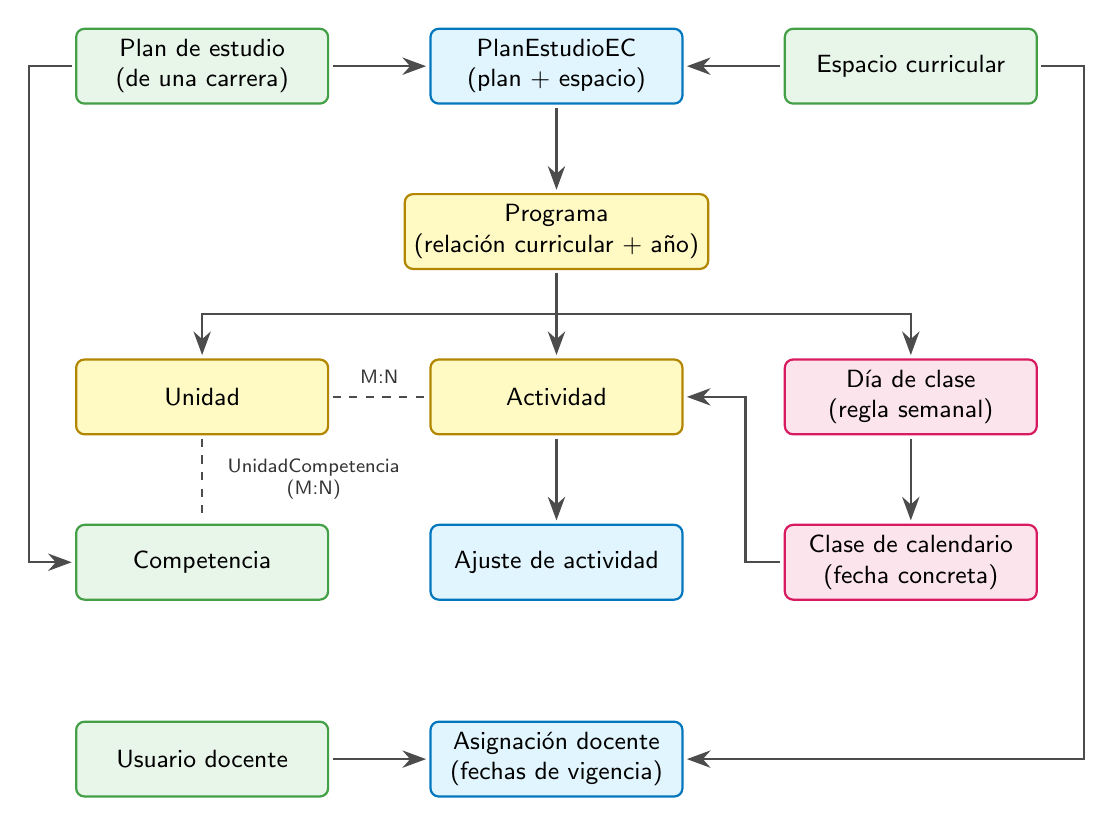
\begin{tikzpicture}[
  font=\sffamily\small,
  box/.style={rectangle,rounded corners=3pt,thick,minimum width=3.2cm,minimum height=.95cm,align=center},
  entity/.style={box,draw=greenStroke,fill=greenFill},
  relation/.style={box,draw=coreStroke,fill=coreFill},
  plan/.style={box,draw=procStroke,fill=procFill},
  event/.style={box,draw=optStroke,fill=optFill},
  edge/.style={-{Stealth[length=3mm,width=2.2mm]},line width=.9pt,draw=black!70,shorten >=1.2pt,shorten <=1.2pt},
  many/.style={line width=.9pt,dashed,draw=black!70,shorten >=1.2pt,shorten <=1.2pt},
  label/.style={font=\sffamily\scriptsize,align=center,text=black!80}
]
% Solid arrows run from a referenced entity to related dependent records.
% Dashed lines show many-to-many associations, without a directional claim.
\node[entity] (planest) at (0,0) {Plan de estudio\\(de una carrera)};
\node[relation] (planec) at (4.5,0) {PlanEstudioEC\\(plan + espacio)};
\node[entity] (ec) at (9,0) {Espacio curricular};
\node[plan] (program) at (4.5,-2.1) {Programa\\(relación curricular + año)};
\node[plan] (unit) at (0,-4.2) {Unidad};
\node[plan] (activity) at (4.5,-4.2) {Actividad};
\node[event] (weekly) at (9,-4.2) {Día de clase\\(regla semanal)};
\node[entity] (competency) at (0,-6.3) {Competencia};
\node[relation] (adjustment) at (4.5,-6.3) {Ajuste de actividad};
\node[event] (occurrence) at (9,-6.3) {Clase de calendario\\(fecha concreta)};
\node[entity] (user) at (0,-8.8) {Usuario docente};
\node[relation] (assignment) at (4.5,-8.8) {Asignación docente\\(fechas de vigencia)};

\draw[edge] (planest.east) -- (planec.west);
\draw[edge] (ec.west) -- (planec.east);
\draw[edge] (planec.south) -- (program.north);
\draw[edge] (program.south) -- (activity.north);
\draw[edge] (program.south) -- (4.5,-3.15) -- (0,-3.15) -- (unit.north);
\draw[edge] (program.south) -- (4.5,-3.15) -- (9,-3.15) -- (weekly.north);
\draw[many] (unit.east) -- (activity.west);
\node[label] at (2.25,-3.95) {M:N};
\draw[many] (unit.south) -- (competency.north);
\node[label,anchor=west] at (.2,-5.25) {UnidadCompetencia\\(M:N)};
\draw[edge] (planest.west) -- (-2.2,0) -- (-2.2,-6.3) -- (competency.west);
\draw[edge] (activity.south) -- (adjustment.north);
\draw[edge] (weekly.south) -- (occurrence.north);
\draw[edge] (occurrence.west) -- (6.9,-6.3) -- (6.9,-4.2) -- (activity.east);
\draw[edge] (user.east) -- (assignment.west);
\draw[edge] (ec.east) -- (11.2,0) -- (11.2,-8.8) -- (assignment.east);
\end{tikzpicture}
\end{document}
